\chapter{Apéndice C. Diagramas de Flujo del Mando Central.}

\begin{table}[H]
  \centering
  \caption{Descripción de las funciones adicionales de los diagramas de flujo}
    \begin{tabular}{@{}|c|p{10cm}|}
    \hline
    \textbf{Función} & \textbf{Descripción} \\
    \hline \hline
    \textbf{tiempo()} & Define si es de \textit{día} o de \textit{noche} en función de la hora obtenida. \\
    \hline
    \textbf{humedad()} & Determina si llueve o no en función de la lectura del sensor respectivo. \\
    \hline
    \textbf{espera()} & Temporizador de espera para la siguiente iteración. Puede ser interrumpido si se apaga el robot o si se desea cambiar de modo de operación. \\
    \hline
    \textbf{GPS()} & Obtiene las coordenadas globales del robot, tanto longitud como latitud en función del sensor respectivo. \\
    \hline
    \textbf{archivo()} & Almacena la información obtenida (fecha, hora y ángulos obtenidos) en un archivo de texto para su uso en la Interfaz. Crea un nuevo archivo si se trata de un día diferente al anterior calculado o sobrescribe en el mismo si se sigue en el mismo día.\\
    \hline
    \textbf{prendido()} & Enciende o apaga al robot. \\
    \hline
    \textbf{desicion()} & Cambia el modo de operación. \\
    \hline
    \textbf{presion()} & Mide la presión atmosférica en función de la lectura del sensor respectivo. \\
    \hline
    \textbf{temperatura()} & Mide la temperatura en el ambiente en función de la lectura del sensor respectivo. \\
    \hline
    \end{tabular}%
  \label{tab:dia_flu2}%
\end{table}%

\begin{figure}[H]
	\centering
	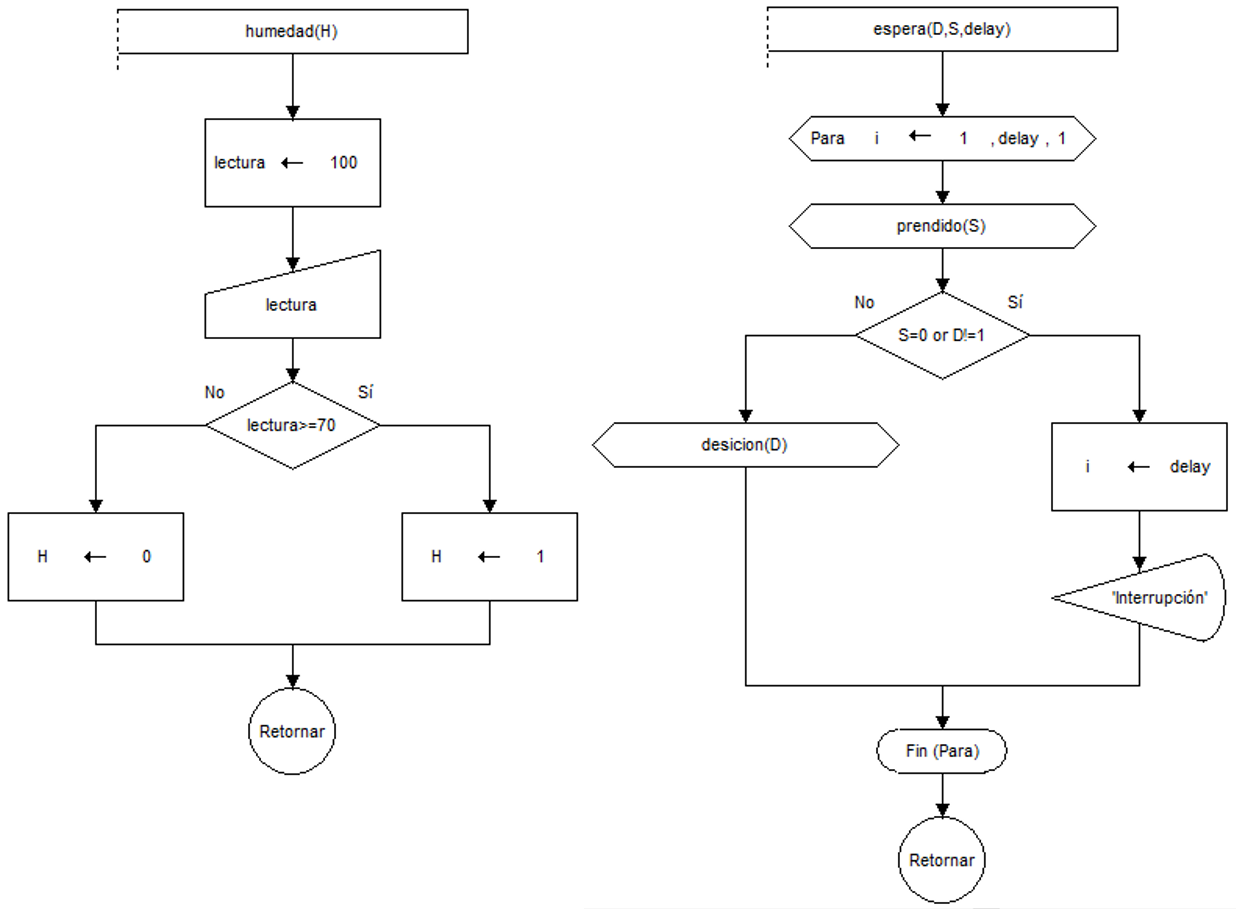
\includegraphics[width=\columnwidth]{imagenes/DF_humedadyespera}
	\caption{Diagramas de flujo de la función \textit{humedad()} y de la función \textit{espera()}}
	\label{fig:dia_fluj5}
\end{figure}

\begin{figure}[H]
	\centering
	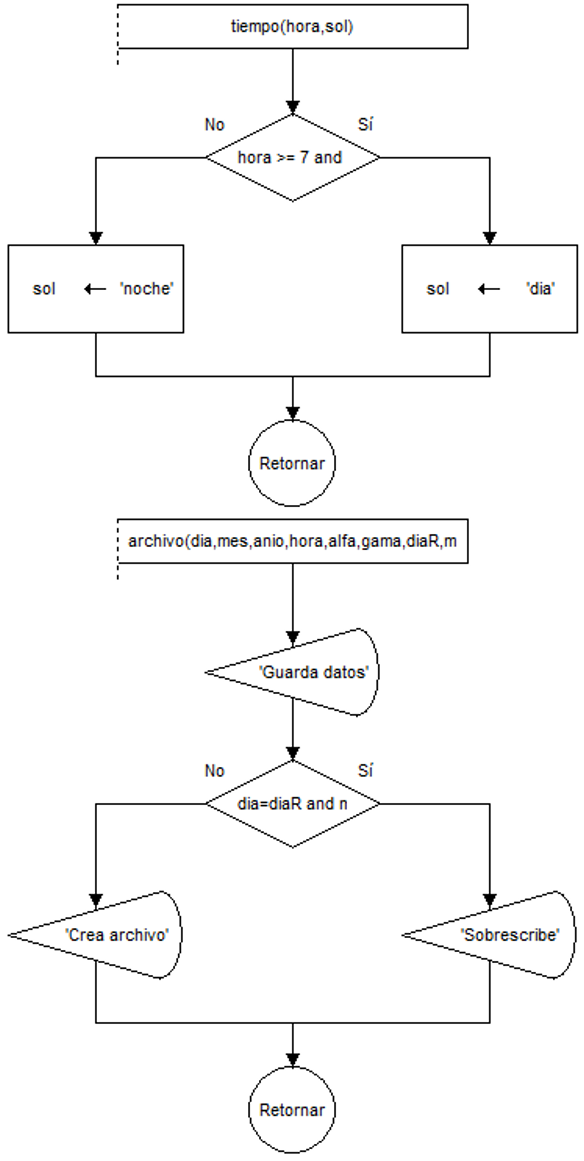
\includegraphics[width=8cm]{imagenes/DF_tiempoyarchivo}
	\caption{Diagramas de flujo de la función \textit{tiempo()} y de la función \textit{archivo()}}
	\label{fig:dia_fluj6}
\end{figure}

\begin{figure}[H]
	\centering
	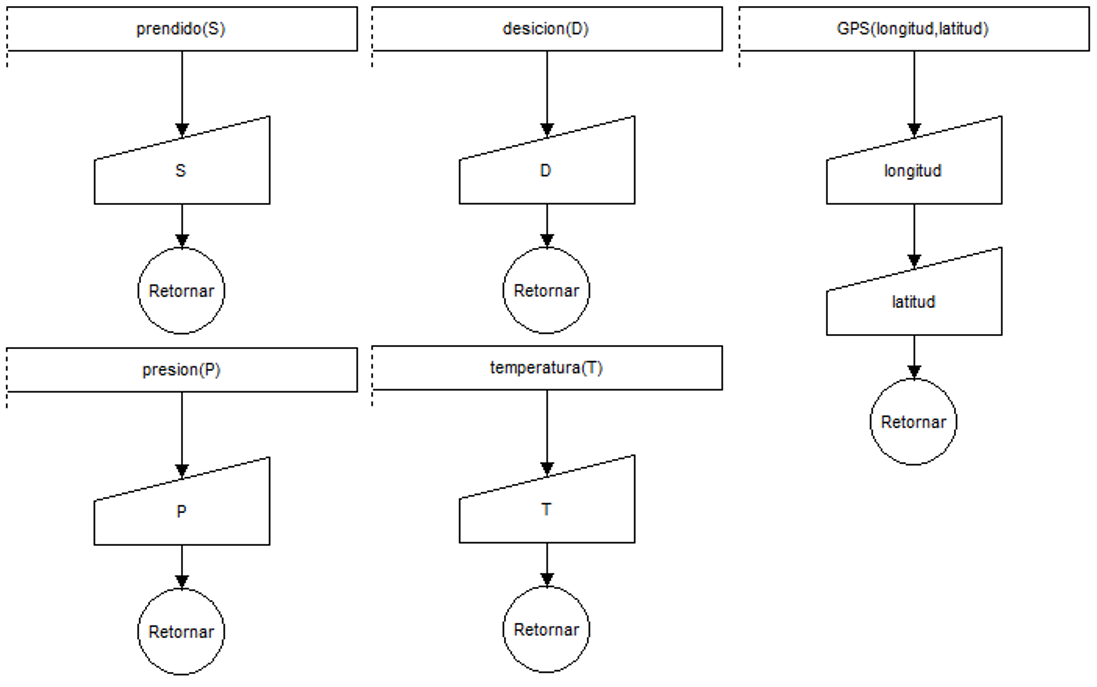
\includegraphics[width=\columnwidth]{imagenes/DFsensores}
	\caption{Diagramas de flujo de los sensores}
	\label{fig:dia_fluj7}
\end{figure}

\bigskip

%%%%%%fin del archivo
\endinput 